% ============================================================================
% Current architecture of the AV2 Hybrid LLM Predictor (exp11 state)
% Source of truth: simpl/hybrid_llm_model.py, simpl/av2_llm_loss.py
% Compile: pdflatex model_architecture.tex   (standalone, no CJK needed)
%
% Key facts encoded in this figure:
%   * The LLM does NOT predict trajectories. It outputs per-agent hidden
%     states (AGT positions) that become a zero-init residual CORRECTION
%     added to the numeric AgentEncoder embedding.
%   * Trajectories are decoded by the Bezier MLP decoder inside the
%     Level-k InteractionDecoder.
%   * Mode queries are anchor-tied: mode k = base_q[k] + MLP(anchor_k),
%     with anchors from an EMA codebook of GT endpoints (no grad).
%   * Scissors = detach points; "0-init" = zero-initialised residual.
% ============================================================================
\documentclass[tikz,border=10pt]{standalone}
\usetikzlibrary{positioning,fit,arrows.meta,calc,backgrounds}
\usepackage{amsmath}
\usepackage{pifont}
\newcommand{\scissors}{\ding{34}}

\tikzset{
  box/.style       ={draw, rounded corners=2pt, align=center, font=\small,
                     inner sep=4pt, minimum height=7mm},
  enc/.style       ={box, fill=blue!12},
  llm/.style       ={box, fill=orange!20},
  dec/.style       ={box, fill=green!15},
  nograd/.style    ={box, fill=gray!15, dashed},
  lossbox/.style   ={box, fill=red!12},
  data/.style      ={align=center, font=\scriptsize\itshape},
  arr/.style       ={-{Stealth[length=2.5mm]}, thick},
  resid/.style     ={arr, blue!60!black, dashed},
  nogradarr/.style ={arr, gray, dash dot},
  lbl/.style       ={font=\scriptsize, midway, fill=white, inner sep=1pt},
  cut/.style       ={font=\footnotesize, text=red},
}

\begin{document}
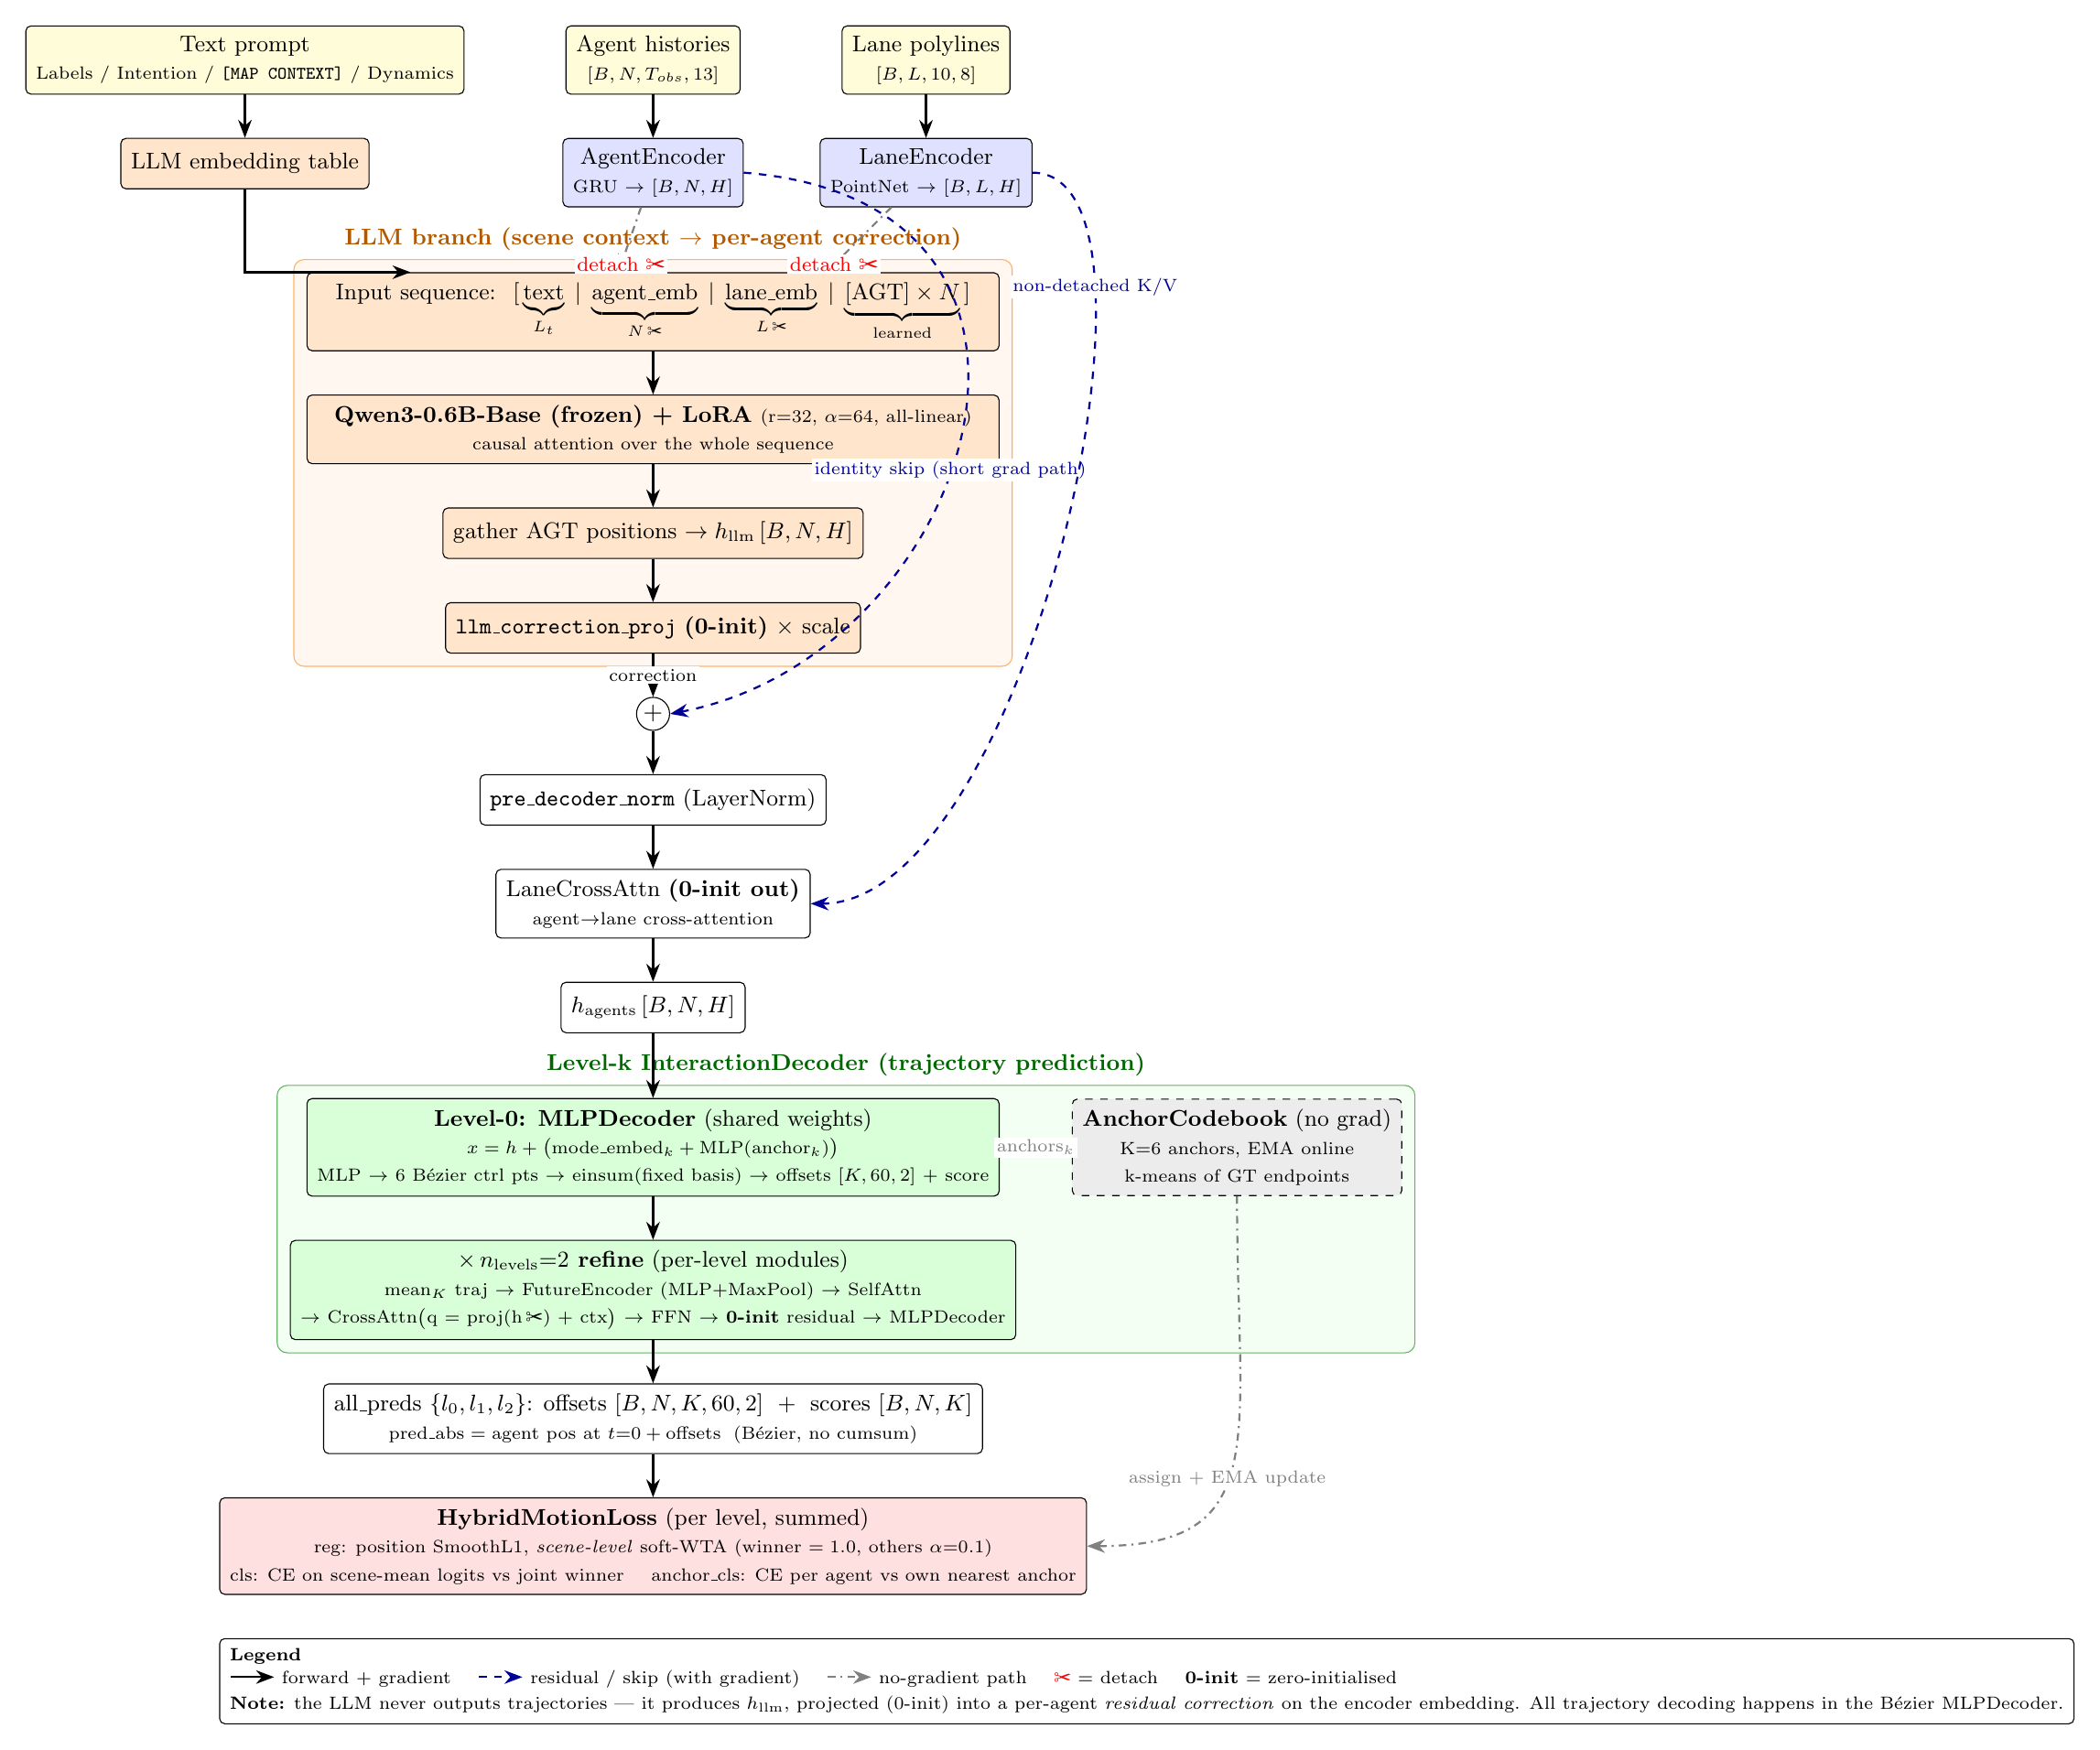
\begin{tikzpicture}[node distance=6mm and 8mm]

% ── Inputs ───────────────────────────────────────────────────────────────
\node[box, fill=yellow!15] (text) {Text prompt\\ \scriptsize Labels / Intention / \texttt{[MAP CONTEXT]} / Dynamics};
\node[box, fill=yellow!15, right=14mm of text] (agentin) {Agent histories\\ \scriptsize $[B,N,T_{obs},13]$};
\node[box, fill=yellow!15, right=14mm of agentin] (lanein) {Lane polylines\\ \scriptsize $[B,L,10,8]$};

% ── Encoders ─────────────────────────────────────────────────────────────
\node[llm, below=of text]    (embed)   {LLM embedding table};
\node[enc, below=of agentin] (agentenc){AgentEncoder\\ \scriptsize GRU $\to$ $[B,N,H]$};
\node[enc, below=of lanein]  (laneenc) {LaneEncoder\\ \scriptsize PointNet $\to$ $[B,L,H]$};

% ── LLM input sequence ───────────────────────────────────────────────────
\node[llm, below=9mm of agentenc, minimum width=96mm] (seq)
  {Input sequence:\;
   $[\,\underbrace{\text{text}}_{L_t}\;|\;
      \underbrace{\text{agent\_emb}}_{N\,\text{\scissors}}\;|\;
      \underbrace{\text{lane\_emb}}_{L\,\text{\scissors}}\;|\;
      \underbrace{\text{[AGT]}\times N}_{\text{learned}}\,]$};

\node[llm, below=of seq, minimum width=96mm] (qwen)
  {\textbf{Qwen3-0.6B-Base (frozen) + LoRA} \scriptsize(r=32, $\alpha$=64, all-linear)\\
   \scriptsize causal attention over the whole sequence};

\node[llm, below=of qwen] (hllm)
  {gather AGT positions $\to h_{\mathrm{llm}}\,[B,N,H]$};

\node[llm, below=of hllm] (corr)
  {\texttt{llm\_correction\_proj} \textbf{(0-init)} $\times$ scale};

% ── Residual fusion ──────────────────────────────────────────────────────
\node[circle, draw, inner sep=1pt, below=of corr] (plus) {$+$};
\node[box, below=of plus] (prenorm) {\texttt{pre\_decoder\_norm} (LayerNorm)};
\node[box, below=of prenorm] (lanex)
  {LaneCrossAttn \textbf{(0-init out)}\\ \scriptsize agent$\to$lane cross-attention};
\node[box, below=of lanex] (hagents) {$h_{\mathrm{agents}}\,[B,N,H]$};

% ── Interaction decoder ─────────────────────────────────────────────────
\node[dec, below=9mm of hagents, minimum width=70mm] (level0)
  {\textbf{Level-0: MLPDecoder} (shared weights)\\
   \scriptsize $x = h + \big(\text{mode\_embed}_k + \text{MLP}(\text{anchor}_k)\big)$\\
   \scriptsize MLP $\to$ 6 B\'ezier ctrl pts $\to$ einsum(fixed basis) $\to$ offsets $[K,60,2]$ + score};

\node[dec, below=of level0, minimum width=70mm] (refine)
  {\textbf{$\times\,n_{\mathrm{levels}}{=}2$ refine} (per-level modules)\\
   \scriptsize mean$_K$ traj $\to$ FutureEncoder (MLP+MaxPool) $\to$ SelfAttn\\
   \scriptsize $\to$ CrossAttn\big(q = \text{proj}(h\,\text{\scissors}) + \text{ctx}\big) $\to$ FFN $\to$ \textbf{0-init} residual $\to$ MLPDecoder};

% ── Anchor codebook (no grad) ────────────────────────────────────────────
\node[nograd, right=10mm of level0, minimum width=34mm] (codebook)
  {\textbf{AnchorCodebook} (no grad)\\
   \scriptsize K=6 anchors, EMA online\\ \scriptsize k-means of GT endpoints};

% ── Outputs & loss ────────────────────────────────────────────────────────
\node[box, below=of refine] (out)
  {all\_preds $\{l_0,l_1,l_2\}$: offsets $[B,N,K,60,2]$ \;+\; scores $[B,N,K]$\\
   \scriptsize $\mathrm{pred\_abs} = \text{agent pos at } t{=}0 + \text{offsets}$ \;(B\'ezier, no cumsum)};

\node[lossbox, below=of out, minimum width=96mm] (loss)
  {\textbf{HybridMotionLoss} (per level, summed)\\
   \scriptsize reg: position SmoothL1, \emph{scene-level} soft-WTA (winner $=1.0$, others $\alpha{=}0.1$)\\
   \scriptsize cls: CE on scene-mean logits vs joint winner \quad
   anchor\_cls: CE per agent vs own nearest anchor};

% ── Main flow arrows ──────────────────────────────────────────────────────
\draw[arr] (text)     -- (embed);
\draw[arr] (agentin)  -- (agentenc);
\draw[arr] (lanein)   -- (laneenc);
\draw[arr] (embed)    |- ($(seq.north west)!.15!(seq.north east)$);
\draw[nogradarr] (agentenc) -- node[lbl, cut, pos=.88] {detach \scissors} ($(seq.north west)!.45!(seq.north east)$);
\draw[nogradarr] (laneenc)  -- node[lbl, cut, pos=.88] {detach \scissors} ($(seq.north west)!.75!(seq.north east)$);
\draw[arr] (seq)   -- (qwen);
\draw[arr] (qwen)  -- (hllm);
\draw[arr] (hllm)  -- (corr);
\draw[arr] (corr)  -- node[lbl] {correction} (plus);
\draw[arr] (plus)  -- (prenorm);
\draw[arr] (prenorm) -- (lanex);
\draw[arr] (lanex) -- (hagents);
\draw[arr] (hagents) -- (level0);
\draw[arr] (level0) -- (refine);
\draw[arr] (refine) -- (out);
\draw[arr] (out)    -- (loss);

% identity skip: AgentEncoder bypasses the LLM entirely
\draw[resid] (agentenc.east) .. controls +(5.2,-0.4) and +(4.2,0.8) ..
  node[lbl, pos=.55] {identity skip (short grad path)} (plus.east);

% LaneEncoder direct (non-detached) path into LaneCrossAttn
\draw[resid] (laneenc.east) .. controls +(2.2,0) and +(3.0,0) ..
  node[lbl, pos=.25] {non-detached K/V} (lanex.east);

% codebook into decoder queries and loss (no grad)
\draw[nogradarr] (codebook.west) -- node[lbl] {anchors$_k$} (level0.east);
\draw[nogradarr] (codebook.south) .. controls +(0,-3.4) and +(2.6,0) ..
  node[lbl, pos=.55] {assign + EMA update} (loss.east);

% legend
\node[draw, rounded corners=2pt, align=left, font=\scriptsize, anchor=north west,
      inner sep=4pt] at ($(loss.south west)+(0,-6mm)$) (legend)
  {\textbf{Legend}\\[1pt]
   \tikz{\draw[arr] (0,0)--(0.6,0);} forward + gradient \quad
   \tikz{\draw[resid] (0,0)--(0.6,0);} residual / skip (with gradient) \quad
   \tikz{\draw[nogradarr] (0,0)--(0.6,0);} no-gradient path \quad
   \textcolor{red}{\scissors} = detach \quad \textbf{0-init} = zero-initialised\\[2pt]
   \textbf{Note:} the LLM never outputs trajectories --- it produces $h_{\mathrm{llm}}$,
   projected (0-init) into a per-agent \emph{residual correction} on the encoder
   embedding. All trajectory decoding happens in the B\'ezier MLPDecoder.};

% ── background grouping ──────────────────────────────────────────────────
\begin{scope}[on background layer]
  \node[fit=(seq)(qwen)(hllm)(corr), draw=orange!60, rounded corners=4pt,
        fill=orange!6, inner sep=5pt, label={[orange!70!black,font=\small\bfseries]90:LLM branch (scene context $\to$ per-agent correction)}] {};
  \node[fit=(level0)(refine)(codebook), draw=green!50!black!60, rounded corners=4pt,
        fill=green!5, inner sep=5pt, label={[green!40!black,font=\small\bfseries]90:Level-k InteractionDecoder (trajectory prediction)}] {};
\end{scope}

\end{tikzpicture}
\end{document}
